\chapter{Analisi del caso di studio}
\section{Introduzione}
In questo capitolo ci dedicheremo a dare uno sguardo all'architettura prototipale proposta come prodotto del tirocinio curriculare. Forniremo una panoramica generale dell'architettura, descrivendo i progetti che costituiscono la soluzione complessiva ("progetto" e "soluzione" appartengono alla terminologia specifica nel contesto di uno sviluppo di Visual Studio in ambiente .NET) e il loro ruolo rispetto al resto dell'architettura. Si avrà inoltre cura di giustificare le scelte implementative effettuate, con riferimento a o in contrasto con alla teoria e i principi di progettazione esposti nel terzo capitolo. Si ribadisce infatti come la soluzione proposta sia un prototipo, e in quanto tale devia consapevolmente dall'idea platonica del prodotto adatto alla produzione per assecondare vincoli di tempo e risorse inevitabili in un contesto di sviluppo con finalità didattiche. Nei casi in cui un aspetto dell'implementazione si discosti dai principi di buona progettazione delle architetture a microservizi, verrà prontamente indicato l'approccio che, in un contesto di sviluppo professionale, si sarebbe invece adottato, eventualmente descrivendo i \emph{trade-off} dell'impiego dell'una o dell'altra implementazione.

\section{Panoramica della soluzione}
La soluzione complessiva si articola in quattro progetti principali, realizzati con tecnologia \emph{ASP.NET Core}, che rappresentano i microservizi forniti dall'architettura, e tre progetti secondari, che rappresentano rispettivamente una libreria di utility, un progetto condiviso .NET Core per la definizione di modelli di dati condivisi, e il progetto Docker Compose per la gestione automatica e centralizzata dei container che ospitano i microservizi.

Si segnala nella struttura descritta una scelta di progettazione, consciamente non in linea con i principi di incapsulamento e indipendenza dei microservizi, effettuata per snellire un'architettura che sarebbe altrimenti eccessivamente complessa per il numero di servizi principali forniti.
Una progettazione più rigorosa avrebbe richiesto un microservizio a sé stante che ospitasse il motore di generazione di reportistica ed esponesse il servizio verso i microservizi a gestione del client MVC e della Web API. Si è invece optato per l'inclusione del motore di reportistica all'interno del microservizio per la Web API: la generazione di nuovi report è infatti limitata a tale container (il client MVC esegue un redirecting verso di esso, così da non esporre al browser endpoint diversi con lo stesso scopo finale), mentre l'accesso al sistema di storage dei report è condiviso mediante un \emph{named volume} Docker, a sottolineare la provvisorietà di tale soluzione nel contesto di un progetto con prospettive di sviluppo in direzione di un deploy in ambienti distribuiti.

\begin{figure}[H]
    \centering
    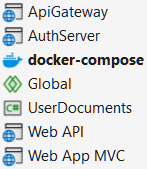
\includegraphics[width=0.4\textwidth]{fig/elenco_progetti.png}
    \caption{Elenco dei progetti che compongono il codice sorgente della soluzione}
\end{figure}